% CVPR 2024 Paper Template; see https://github.com/cvpr-org/author-kit

\documentclass[10pt,twocolumn,letterpaper]{article}

%%%%%%%%% PAPER TYPE  - PLEASE UPDATE FOR FINAL VERSION
\usepackage{cvpr}              % To produce the CAMERA-READY version
% \usepackage[review]{cvpr}      % To produce the REVIEW version
% \usepackage[pagenumbers]{cvpr} % To force page numbers, e.g. for an arXiv version
% Import additional packages in the preamble file, before hyperref
%
% --- inline annotations
%
\usepackage[dvipsnames, table]{xcolor}
\usepackage{tabularx}
\usepackage{longtable}
\usepackage{array}
\usepackage{multicol}
\newcommand{\red}[1]{{\color{red}#1}}
\newcommand{\todo}[1]{{\color{red}#1}}
\newcommand{\TODO}[1]{\textbf{\color{red}[TODO: #1]}}
% --- disable by uncommenting  
% \renewcommand{\TODO}[1]{}
% \renewcommand{\todo}[1]{#1}


% It is strongly recommended to use hyperref, especially for the review version.
% hyperref with option pagebackref eases the reviewers' job.
% Please disable hyperref *only* if you encounter grave issues, 
% e.g. with the file validation for the camera-ready version.
%
% If you comment hyperref and then uncomment it, you should delete *.aux before re-running LaTeX.
% (Or just hit 'q' on the first LaTeX run, let it finish, and you should be clear).
\definecolor{cvprblue}{rgb}{0.21,0.49,0.74}
\definecolor{myblue}{rgb}{0.0,0.45,0.74}
% \usepackage[pagebackref,breaklinks,colorlinks,citecolor=cvprblue]{hyperref}
\usepackage[hidelinks]{hyperref}

% \usepackage{lipsum}% http://ctan.org/pkg/lipsum
% \usepackage{multicol}% http://ctan.org/pkg/multicols
% \usepackage{balance}

\usepackage{graphicx}
\graphicspath{ {./images/} }

%%%%%%%%% PAPER ID  - PLEASE UPDATE
\def\paperID{*****} % *** Enter the Paper ID here
\def\confName{CVPR}
\def\confYear{2024}

%%%%%%%%% TITLE - PLEASE UPDATE
\title{Fusion Modeling \& Knowledge Distillation Optimization for Video-Based Cardiac Monitoring}

%%%%%%%%% AUTHORS - PLEASE UPDATE
\author{Wangshui Kang\\
ID: A20500653\\
{\tt\small wkang10@hawk.iit.edu}
\and
Junhui Zhan\\
ID: A20499169\\
{\tt\small jzhan4@hawk.iit.edu}
\and
Sidi Li\\
ID: A20479715\\
{\tt\small sli178@hawk.iit.edu}
}

\begin{document}
\maketitle
\begin{abstract}
Despite significant advancements in the prevention and diagnosis of cardiovascular disease in recent years, heart disease remains the leading cause of adult mortality worldwide. This is partly attributed to the vital role played by blood circulation in facilitating oxygen-carbon dioxide exchange among most organs within the body. Consequently, any abnormality in the heart's pumping capacity can lead to irreversible damage across multiple organs within a short timeframe (3-8 minutes).

However, current human assessment of cardiac function primarily focuses on limited monitoring of cardiac beat cycles and specialized blood tests. The measurement of left ventricular ejection fraction (the ratio between changes in left ventricular end-systolic volume and left ventricular end-diastolic volume) stands as one of the most crucial indicators for evaluating cardiac function.

But the traditional measurement of the heart's left ventricular ejection fraction (LVEF) by ultrasound instrumentation is not the gold standard, and is hardly the gold standard. Because the measurement of EF by ultrasound is always semi-quantitative, the value of the measurement appears to be objective, but the operator who performs the measurement is subjective. In the clinical process, it is often found that different operators measure the EF of the same patient, but the results are very different, and even the same operator for the same patient EF measurement, but also get different results. So, how can we obtain as accurate an EF as possible to guide the diagnosis and treatment plan during clinical diagnosis and treatment?
\end{abstract}

\section{Brief Survey}
\label{sec:intro}

Discrepancies observed during ejection fraction assessments are partially due to common heart rate irregularities and computational challenges associated with manually tracking ventricular size for each beat. Additionally, physiological differences age, chest size, working and living environments, as well as behavioral habits contribute to variations in the basic contour of the heart even when examining individuals with normal physiological functions. Furthermore, different angles used during testing by non-cardiologists utilizing point-of-care ultrasound can significantly impact results.

Even after extensive training, physicians may still exhibit substantial divergent biases or omissions when assessing emergencies or rare diseases. Such discrepancies pose potential dangers alike. Therefore, there is an urgent need for rapid, efficient, cost-effective, accurate, reproducible, and quantifiable methods for assessing cardiac function.

\section{Proposed work}
The acquisition of echocardiographic images is rapid, cost-effective, and free from ionizing radiation, making it the most widely utilized modality in cardiovascular imaging. To address this challenge, we propose "Fusion Modeling  \& Knowledge Distillation Optimization," which leverages a video-based deep learning algorithm called EchoNet-Dynamic. This approach combines feature extraction using multiple models (employing a window-based attention mechanism with multiple convolutional networks, a mixed model that enjoys the benefit of both self-Attention(maybe also Cross-Attention) and Convolution (ACmix), while having minimum computational overhead compared to the pure convolution or selfattention counterpart) and surpasses human experts in critical tasks such as left ventricle segmentation and ejection fraction estimation while significantly reducing computational requirements. Although Knowledge Distillation Optimization can optimize the neural network structure to speed up inference, it comes at the cost of decreased accuracy. Therefore, we hope to compensate for this loss by Attention modeling It is user-friendly, requires minimal or no parameter tuning, and can be executed efficiently on personal computers. Future prospects include extending its application to detect and monitor other organs, tissues, and body behaviors through video analysis to enhance auxiliary clinical diagnosis, treatment planning, and risk assessment. A longer term plan is to realize 3D reconstruction of the entire cardiac activity by means of ultrasound video from multiple angles to achieve a 360-degree view and avoid cross-sectional errors due to the acquisition angle of the ultrasound probe.

\section{Preliminary plan}
\label{sec:formatting}

\noindent
\begin{minipage}{0.5\textwidth}
    \fontsize{7}{10}\selectfont
    \begin{tabular}{|>{\raggedright\arraybackslash}m{1cm}|>{\raggedright\arraybackslash}m{3cm}|c|c|}
        \hline
        \rowcolor{myblue} \color{white} Milestone & \color{white} Content & \color{white} Plan Date & \color{white} Finish Date \\
        \hline
        Setup Dev ENV & Hardware including GPU, PyTorch config ready. & 2023/10/01 & 2023/09/25\\
        \hline
        Get Data & Register and download the dataset via the Stanford Artificial Intelligence in Medicine and Imaging (AIMI) Center Shared Datasets Portal. & 2023/10/01 & 2023/09/25\\
        \hline
        Get Init code & Download EchoNet-Dynamic code from GitHub. & 2023/10/01 & 2023/09/29\\
        \hline
        Run and record base test & Use the step 2 and 3 to get the code run and get expected results. & 2023/10/15 & -\\
        \hline
        Fusion Modeling & Use different methods to build models to get better features. & 2023/10/17 & -\\
        \hline
        Run and record Modeling & Test to find out a good network architecture also the hyper-parameters. & 2023/10/21 & -\\
        \hline
        Intermediate Project Report & Introduction to the problem, data, what has been done so far, what remains to be done. & 2023/10/27 & -\\
        \hline
        Model Optimization & Use Knowledge Distillation to cut down the network. & 2023/11/10 & -\\
        \hline
        Run and record Optimization & Test to find out a good network architecture also the hyper-parameters. & 2023/11/20 & -\\
        \hline
        Analysis and summary for final project report & Summary of the problem, previous work, methods, and results; the problem try to address methodology; observations from the experiments; Conclusions and future work. & 2023/11/28 & -\\
        \hline
        Final Project Presentation & 5-8 minutes; Describe the motivation and problem description; Briefly present the intuition behind the technical details (methodology); Algorithm and results (you can use a demo). & 2023/11/28 & -\\
        \hline
    \end{tabular}
\end{minipage}%
\section{Description of the dataset}

A standard full resting echocardiogram study consists of a series of 50–100 videos and still images visualizing the heart from different angles, locations and image acquisition techniques (two-dimensional images, tissue Doppler images, color Doppler images and others). Each echocardiogram video corresponds to a unique patient and a unique visit. In this dataset, one apical four-chamber two-dimensional greyscale video is extracted from each study. Each video represents a unique individual as the dataset contains 10,030 echocardiography videos from 10,030 unique individuals who underwent echocardiography between 2016 and 2018 as part of clinical care at Stanford Health Care. Videos were randomly split into 7,465, 1,277 and 1,288 patients, respectively, for the training, validation and test sets.

The randomly selected patients in our data have a range of ejection fractions representative of the patient population who visit the echocardiography laboratory. Videos were acquired by skilled sonographers using iE33, Sonos, Acuson SC2000, Epiq 5G or Epiq 7C ultrasound machines and processed images were stored in a Philips Xcelera picture archiving and communication system. Video views were identified through implicit knowledge of view classification in the clinical database by identifying images and videos labelled with measurements done in the corresponding view. For example, apical four-chamber videos were identified by selecting videos from the set of videos in which a sonographer or cardiologist traced left ventricle volumes and labelled these for analysis to calculate ejection fraction. The apical four-chamber view video was thus identified by extracting the Digital Imaging and Communications in Medicine (DICOM) file linked to the measurements of the ventricular volume used to calculate the ejection fraction.

An automated preprocessing workflow was used to remove identifying information and eliminate unintended human labels. Each subsequent video was cropped and masked to remove text, electrocardiogram and respirometer information, and other information outside of the scanning sector. The resulting square images were either 600 × 600 or 768 × 768 pixels depending on the ultrasound machine and down sampled by cubic interpolation using OpenCV into standardized 112 × 112 pixel videos. Videos were spot-checked for quality control, to confirm view classification and to exclude videos with color Doppler.

This research was approved by the Stanford University Institutional Review Board and data privacy review through a standardized workflow by the Center for Artificial Intelligence in Medicine and Imaging (AIMI) and the University Privacy Office. In addition to masking of text, electrocardiogram information and extra data outside of the scanning sector in the video files as described above, the video data of each DICOM file was saved as an AVI file to prevent any leakage of identifying information through public or private DICOM tags. Each video was subsequently manually reviewed by an employee of the Stanford Hospital familiar with imaging data to confirm the absence of any identifying information before public release.


\vfill
\section{Workflow}

\begin{figure*}[h]
\centering
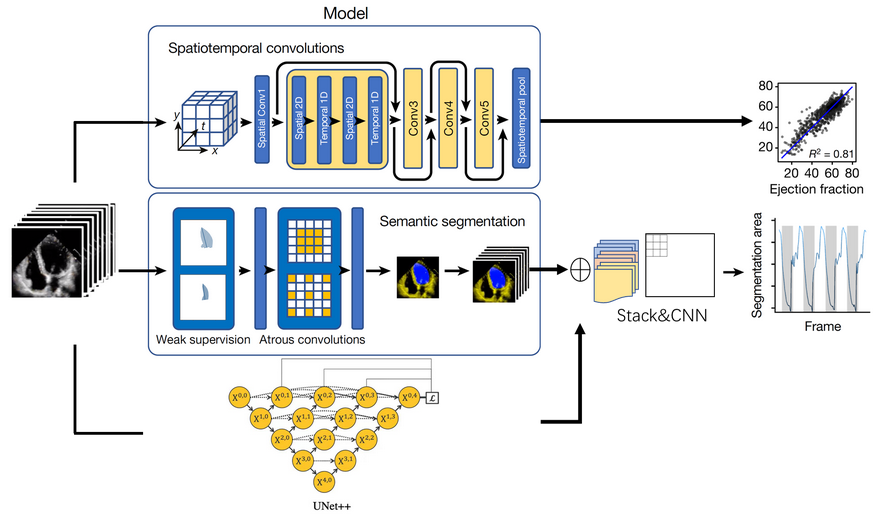
\includegraphics[width=0.9\textwidth]{workflow}
\caption{EchoNet-Dynamic architecture}
\label{EchoNet-Dynamic}
\end{figure*}

EchoNet-Dynamic has three key components(Figure \ref{EchoNet-Dynamic}). First, it constructed a CNN model with atrous convolutions for frame-level semantic segmentation of the left ventricle. The technique of atrous convolutions enables the model to capture larger patterns and has previously been shown to perform well on non-medical imaging datasets.The standard human clinical workflow for estimating the ejection fraction requires manual segmentation of the left ventricle during end systole and end diastole. We generalize these labels in a weak supervision approach with atrous convolutions to generate frame-level semantic segmentation throughout the cardiac cycle in a 1:1 pairing with frames from the original video. The automatic segmentation is used to identify ventricular contractions and provides a clinician-interpretable intermediary that mimics the clinical workflow.

Second, it trained a CNN model with residual connections and spatiotemporal convolutions across frames to predict the ejection fraction. In contrast to previous CNN architectures for machine learning of medical images, our approach integrates spatial as well as temporal information in our network convolutions. Spatiotemporal convolutions,which incorporate spatial information in two dimensions as well as temporal information in the third dimension, have previously been used in non-medical video-classification tasks. However, this approach has not previously been used for medical data given the relative scarcity of labelled medical videos.

In EchoNet-Dynamic's architecture, integrating UNet++ with a three-layer design alongside DeepLabV3 is aimed to enhance model performance. UNet++ optimizes semantic segmentation through dense skip connections, capturing more contextual information and reducing information loss. By concatenating this with DeepLabV3, we aim to combine their segmentation strengths, especially in detailing left ventricle structures, to improve ejection fraction estimation accuracy. This integration seeks to enrich contextual understanding crucial for analyzing cardiac function, thereby aiming to optimize EchoNet-Dynamic's reliability in cardiac function assessment.

Finally, it makes video-level predictions of the ejection fraction for beat-to-beat estimations of cardiac function. Given that variation in cardiac function can be caused by changes in loading conditions as well as heart rate in a variety of cardiac conditions, it is recommended to perform estimations of the ejection fraction for up to five cardiac cycles; however, this is not always done in clinical practice given the tedious and laborious nature of the calculation. Our model identifies each cardiac cycle, generates a clip of 32 frames and averages clip-level estimates of the ejection fraction for each beat as test-time augmentation. EchoNet-Dynamic was developed using 10,030 apical four-chamber echocardiogram videos obtained during the course of routine clinical practice at Stanford Medicine.

\vfill
\section{Development and training}

Model design and training was done in Python using the PyTorch deep learning library. Semantic segmentation was performed using the Deeplabv3 architecture. The segmentation model had a base architecture of a 101-layer residual net and minimized pixel-level binary crossentropy loss. The model was initialized with random weights and was trained using a stochastic gradient descent optimizer. We assessed three model architectures with variable integration of temporal convolutions (R3D, MC3 and R2+1D) and ultimately chose decomposed R2+1D spatiotemporal convolutions as the architecture with the best performance to use for EchoNet-Dynamic. In the R3D architecture, all convolutional layers considered the spatial and temporal dimensions jointly and these consisted of five convolutional blocks. The MC3 and R2+1D architectures were introduced as a middle ground between two-dimensional convolutions that considered only spatial relationships and the full three-dimensional convolutions used by R3D. The MC3 architecture replaced the convolutions in the final three blocks with two-dimensional convolutions, and the R2+1 architecture explicitly factored all of the three-dimensional convolutions into a two-dimensional spatial convolution followed by a one-dimensional temporal convolution.

In the model design and training phase, we integrated the UNet++ architecture to enhance performance. We dissected the Deeplabv3 architecture from torchvision, added transformation layers to the backbone, and connected it with the UNet++ network. The output of this new network was then connected with a classifier, forming our new model. This integration aims to achieve more accurate semantic segmentation and better results in predicting ejection fraction for EchoNet-Dynamic.

For predicting ejection fraction, the models were trained to minimize the squared loss between the prediction and true ejection fraction using a stochastic gradient descent optimizer with an initial learning rate of 0.0001, momentum of 0.9 and batch size of 16 for 45 epochs. The learning rate was decayed by a factor of 0.1 every 15 epochs. For model input, video clips of 32 frames were generated by sampling every other frame (sampling period of 2) with both clip length and sampling period determined by hyperparameter search. During training, to augment the size of the dataset and increase the variation of exposed training clips, each training video clip was padded with 12 pixels on each side, and a random crop of the original frame size was taken to simulate slight translations and changes in camera location. For all models, the weights from the epoch with the lowest validation loss was selected for final testing. Model computational using one NVIDIA GeForce RTX 4070 Ti GPU.

\vfill
\section{Evaluation of model performance}

For the test dataset from Stanford Medicine that was not previously seen during model training, the prediction of the ejection fraction by EchoNet-Dynamic had a mean absolute error of 4.1\%, root mean squared error of 5.3\% and R2 of 0.81 compared with the annotations by human experts. This is well within the range of typical measurement variation between different clinicians, which is usually described as inter-observer variation and can be as high as 13.9\%. Wait for result

%\section{Statistical analysis}

No statistical methods were used to predetermine sample size. Confidence intervals were computed using 10,000 bootstrapped samples and obtaining 95 percentile ranges for each prediction. The performance of the semantic segmentation task was evaluated using the Dice similarity coefficient compared with the human labels from the held-out test dataset. The performance of the ejection fraction task was evaluated by calculating the mean absolute difference between the prediction of EchoNet-Dynamic and the human calculation of ejection fraction as well as calculating the R2 between the prediction by EchoNet-Dynamic and the human calculation. Prospective comparison with human readers was performed with the uniformly most powerful invariant equivalence test for two-sample problems.


\section{Reference}

\begin{itemize}
  \item Video-based AI for beat-to-beat assessment of cardiac function 
Paper Published: 25 March 2020
\url{https://www.nature.com/articles/s41586-020-2145-8} (need to pay but we've already paid to download it)
  \item EchoNet-Dynamic \url{https://echonet.github.io/dynamic/}
  \item EchoNet-Dynamic Code: \url{https://github.com/echonet/dynamic}
  \item EchoNet-Dynamic	 Data:7.04 GB, December 2020
Access the dataset via the Stanford Artificial Intelligence in Medicine and Imaging (AIMI) Center Shared Datasets Portal. Pls registor and follow the rules.
  \item ACmix  \url{https://github.com/LeapLabTHU/ACmix}
  \item U-Net \url{https://arxiv.org/abs/1505.04597}
  \item Deeplab \url{https://arxiv.org/abs/1412.7062}
  \item Knowledge distillation \url{https://en.wikipedia.org/wiki/Knowledge_distillation}
  \item On the Integration of Self-Attention and Convolution  \url{https://arxiv.org/pdf/2111.14556.pdf}
  \item \url{https://download.csdn.net/blog/column/12194563/129044015}
  \item \url{https://zhuanlan.zhihu.com/p/539706748}
  \item \url{https://zhuanlan.zhihu.com/p/539740657}
  \item \url{https://zhuanlan.zhihu.com/p/608312950?utm_id=0&wd=&eqid=c37be367000f6cbf000000066486c9ce}
  \item \url{https://stanfordaimi.azurewebsites.net/}
  \item \url{https://www.ngui.cc/el/2485409.html?action=onClick}
  \item \url{https://blog.csdn.net/qq_40280673/article/details/127449624}
  \item \url{https://zhuanlan.zhihu.com/p/640904026}
  \item \url{https://aisle.hzau.edu.cn/info/1097/1412.htm}
  \item \url{https://blog.csdn.net/zuzhiang/article/details/107418459}
\end{itemize}

{
    \small
    \bibliographystyle{ieeenat_fullname}
}

% WARNING: do not forget to delete the supplementary pages from your submission 
% \clearpage
\setcounter{page}{1}
\maketitlesupplementary


\section{Rationale}
\label{sec:rationale}
% 
Having the supplementary compiled together with the main paper means that:
% 
\begin{itemize}
\item The supplementary can back-reference sections of the main paper, for example, we can refer to \cref{sec:intro};
\item The main paper can forward reference sub-sections within the supplementary explicitly (e.g. referring to a particular experiment); 
\item When submitted to arXiv, the supplementary will already included at the end of the paper.
\end{itemize}
% 
To split the supplementary pages from the main paper, you can use \href{https://support.apple.com/en-ca/guide/preview/prvw11793/mac#:~:text=Delete%20a%20page%20from%20a,or%20choose%20Edit%20%3E%20Delete).}{Preview (on macOS)}, \href{https://www.adobe.com/acrobat/how-to/delete-pages-from-pdf.html#:~:text=Choose%20%E2%80%9CTools%E2%80%9D%20%3E%20%E2%80%9COrganize,or%20pages%20from%20the%20file.}{Adobe Acrobat} (on all OSs), as well as \href{https://superuser.com/questions/517986/is-it-possible-to-delete-some-pages-of-a-pdf-document}{command line tools}.


\end{document}
